\documentclass[12pt,a4paper]{article}
	%[fleqn] %%% --to make all equation left-algned--

% \usepackage[utf8]{inputenc}
% \DeclareUnicodeCharacter{1D12A}{\doublesharp}
% \DeclareUnicodeCharacter{2693}{\anchor}
% \usepackage{dingbat}
% \DeclareRobustCommand\dash\unskip\nobreak\thinspace{\textemdash\allowbreak\thinspace\ignorespaces}
\usepackage[top=2in, bottom=1in, left=1in, right=1in]{geometry}
%\usepackage{fullpage}

\usepackage{fancyhdr}\pagestyle{fancy}\rhead{Stephanie Wang}\lhead{EE236B Homework 1}

\usepackage{amsmath,amssymb,amsthm,amsfonts,microtype,stmaryrd}
	%{mathtools,wasysym,yhmath}

\usepackage[usenames,dvipsnames]{xcolor}
\newcommand{\blue}[1]{\textcolor{blue}{#1}}
\newcommand{\red}[1]{\textcolor{red}{#1}}
\newcommand{\gray}[1]{\textcolor{gray}{#1}}
\newcommand{\fgreen}[1]{\textcolor{ForestGreen}{#1}}

\usepackage{mdframed}
	%\newtheorem{mdexample}{Example}
	\definecolor{warmgreen}{rgb}{0.8,0.9,0.85}
	% --Example:
	% \begin{center}
	% \begin{minipage}{0.7\textwidth}
	% \begin{mdframed}[backgroundcolor=warmgreen, 
	% skipabove=4pt,skipbelow=4pt,hidealllines=true, 
	% topline=false,leftline=false,middlelinewidth=10pt, 
	% roundcorner=10pt] 
	%%%% --CONTENTS-- %%%%
	% \end{mdframed}\end{minipage}\end{center}	

\usepackage{graphicx} \graphicspath{ {} }
	% --Example:
	% \includegraphics[scale=0.5]{picture name}
%\usepackage{caption} %%% --some awful package to make caption...

%\usepackage{hyperref}\hypersetup{linktocpage,colorlinks}\hypersetup{citecolor=black,filecolor=black,linkcolor=black,urlcolor=black}

%%% --Text Fonts
%\usepackage{times} %%% --Times New Roman for LaTeX
%\usepackage{fontspec}\setmainfont{Times New Roman} %%% --Times New Roman; XeLaTeX only

%%% --Math Fonts
\renewcommand{\v}[1]{\ifmmode\mathbf{#1}\fi}
%\renewcommand{\mbf}[1]{\mathbf{#1}} %%% --vector
%\newcommand{\ca}[1]{\mathcal{#1}} %%% --"bigO"
%\newcommand{\bb}[1]{\mathbb{#1}} %%% --"Natural, Real numbers"
%\newcommand{\rom}[1]{\romannumeral{#1}} %%% --Roman numbers

%%% --Quick Arrows
\newcommand{\ra}[1]{\ifnum #1=1\rightarrow\fi\ifnum #1=2\Rightarrow\fi\ifnum #1=3\Rrightarrow\fi\ifnum #1=4\rightrightarrows\fi\ifnum #1=5\rightleftarrows\fi\ifnum #1=6\mapsto\fi\ifnum #1=7\iffalse\fi\fi\ifnum #1=8\twoheadrightarrow\fi\ifnum #1=9\rightharpoonup\fi\ifnum #1=0\rightharpoondown\fi}

%\newcommand{\la}[1]{\ifnum #1=1\leftarrow\fi\ifnum #1=2\Leftarrow\fi\ifnum #1=3\Lleftarrow\fi\ifnum #1=4\leftleftarrows\fi\ifnum #1=5\rightleftarrows\fi\ifnum #1=6\mapsfrom\ifnum #1=7\iffalse\fi\fi\ifnum #1=8\twoheadleftarrow\fi\ifnum #1=9\leftharpoonup\fi\ifnum #1=0\leftharpoondown\fi}

%\newcommand{\ua}[1]{\ifnum #1=1\uparrow\fi\ifnum #1=2\Uparrow\fi}
%\newcommand{\da}[1]{\ifnum #1=1\downarrow\fi\ifnum #1=2\Downarrow\fi}

%%% --Special Editor Config
\renewcommand{\ni}{\noindent}
\newcommand{\onum}[1]{\raisebox{.5pt}{\textcircled{\raisebox{-1pt} {#1}}}}

\newcommand{\claim}[1]{\underline{``{#1}":}}

\renewcommand{\l}{\left}\renewcommand{\r}{\right}

\newcommand{\casebrak}[2]{\left \{ \begin{array}{l} {#1}\\{#2} \end{array} \right.}
%\newcommand{\ttm}[4]{\l[\begin{array}{cc}{#1}&{#2}\\{#3}&{#4}\end{array}\r]} %two-by-two-matrix
%\newcommand{\tv}[2]{\l[\begin{array}{c}{#1}\\{#2}\end{array}\r]}

\def\dps{\displaystyle}

\let\italiccorrection=\/
\def\/{\ifmmode\expandafter\frac\else\italiccorrection\fi}


%%% --General Math Symbols
\def\bc{\because}
\def\tf{\therefore}

%%% --Frequently used OPERATORS shorthand
\newcommand{\INT}[2]{\int_{#1}^{#2}}
% \newcommand{\UPINT}{\bar\int}
% \newcommand{\UPINTRd}{\overline{\int_{\bb R ^d}}}
\newcommand{\SUM}[2]{\sum\limits_{#1}^{#2}}
\newcommand{\PROD}[2]{\prod\limits_{#1}^{#2}}
\newcommand{\CUP}[2]{\bigcup\limits_{#1}^{#2}}
\newcommand{\CAP}[2]{\bigcap\limits_{#1}^{#2}}
% \newcommand{\SUP}[1]{\sup\limits_{#1}}
% \newcommand{\INF}[1]{\inf\limits_{#1}}
\DeclareMathOperator*{\argmin}{arg\,min}
\DeclareMathOperator*{\argmax}{arg\,max}
\newcommand{\pd}[2]{\frac{\partial{#1}}{\partial{#2}}}
\def\tr{\text{tr}}

\renewcommand{\o}{\circ}
\newcommand{\x}{\times}
\newcommand{\ox}{\otimes}

\newcommand\ie{{\it i.e.}}

%%% --Frequently used VARIABLES shorthand
\def\R{\ifmmode\mathbb R\fi}
\def\N{\ifmmode\mathbb N\fi}
\renewcommand{\O}{\mathcal{O}}

\newcommand{\dt}{\Delta t}
\def\vA{\mathbf{A}}
\def\vB{\mathbf{B}}\def\cB{\mathcal{B}}
\def\vC{\mathbf{C}}
\def\vD{\mathbf{D}}
\def\vE{\mathbf{E}}
\def\vF{\mathbf{F}}\def\tvF{\tilde{\mathbf{F}}}
\def\vG{\mathbf{G}}
\def\vH{\mathbf{H}}
\def\vI{\mathbf{I}}\def\cI{\mathcal{I}}
\def\vJ{\mathbf{J}}
\def\vK{\mathbf{K}}
\def\vL{\mathbf{L}}\def\cL{\mathcal{L}}
\def\vM{\mathbf{M}}
\def\vN{\mathbf{N}}\def\cN{\mathcal{N}}
\def\vO{\mathbf{O}}
\def\vP{\mathbf{P}}
\def\vQ{\mathbf{Q}}
\def\vR{\mathbf{R}}
\def\vS{\mathbf{S}}
\def\vT{\mathbf{T}}
\def\vU{\mathbf{U}}
\def\vV{\mathbf{V}}
\def\vW{\mathbf{W}}
\def\vX{\mathbf{X}}
\def\vY{\mathbf{Y}}
\def\vZ{\mathbf{Z}}

\def\va{\mathbf{a}}
\def\vb{\mathbf{b}}
\def\vc{\mathbf{c}}
\def\vd{\mathbf{d}}
\def\ve{\mathbf{e}}
\def\vf{\mathbf{f}}
\def\vg{\mathbf{g}}
\def\vh{\mathbf{h}}
\def\vi{\mathbf{i}}
\def\vj{\mathbf{j}}
\def\vk{\mathbf{k}}
\def\vl{\mathbf{l}}
\def\vm{\mathbf{m}}
\def\vn{\mathbf{n}}
\def\vo{\mathbf{o}}
\def\vp{\mathbf{p}}
\def\vq{\mathbf{q}}
\def\vr{\mathbf{r}}
\def\vs{\mathbf{s}}
\def\vt{\mathbf{t}}
\def\vu{\mathbf{u}}
\def\vv{\mathbf{v}}\def\tvv{\tilde{\mathbf{v}}}
\def\vw{\mathbf{w}}
\def\vx{\mathbf{x}}\def\tvx{\tilde{\mathbf{x}}}
\def\vy{\mathbf{y}}
\def\vz{\mathbf{z}}

%%% --Numerical analysis related
%\newcommand{\nxt}{^{n+1}}
%\newcommand{\pvs}{^{n-1}}
%\newcommand{\hfnxt}{^{n+\frac12}}

%%%%%%%%%%%%%%%%%%%%%%%%%%%%%%%%%%%%%%%%%%%%%%%%%%%%%%%%%%%%%%%%%%%%%%%%%%%%%%%%%%%%%%%%%%%%%%%%%%%%%%%%%%%%%%%%%%%%%%%%%%%%%%%%%%%%%%%%%%%%%%%%%%%%%%%%%%%%%%%%%%%%%%%%%%%%%%%%%%%%%%%%%%%%%%%%%%%%%%
\begin{document}
\subsubsection*{Exercise 2.7 [Boyd \& Vandenberghe, 2004]}
\noindent {\it Voronoi description of halfspace.} Let $a$ and $b$ be distinct points in $\R^n$. Shpow that the set of all points that are closer (in Euclidean norm) to $a$ than $b$, \ie $\{x \mid  \|x-a\|_2 \leq \|x-b\|_2\}$, is a halfspace. Describe it explicitly as an inequality of the form $c^t x \leq d$. Draw a picture. \\
\\
{\it Ans:} Denote $x = [x_1, \cdots, x_n], a = [a_1, \cdots, a_n], b = [b_1, \cdots, b_n]$, the quiterium $\|x-a\|_2 \leq \|x-b\|_2$ is equivalent to
$$(x_1-a_1)^2 + \cdots + (x_n - a_n)^2 \leq (x_1 - b_1)^2 + \cdots + (x_n - b_n)^2$$
Organize the inequality for a bit (subtract $x_1^2 + \cdots + x_n^2$ for both sides and move terms around) and we get
$$(-2a_1 + 2b_1)x_1 + \cdots + (-2a_n + 2b_n)x_n \leq (b_1^2 -a_1^2) + \cdots + (b_n^2 - a_n^2)$$
Let $c = -a+b \in \R^n$, $d = \/12 (\|b\|_2^2 - \|a\|_2^2) \in \R$ and divide the inequality by $2$, we get
$$c^Tx \leq d$$
as in the desired form.\qed\\
\begin{center}
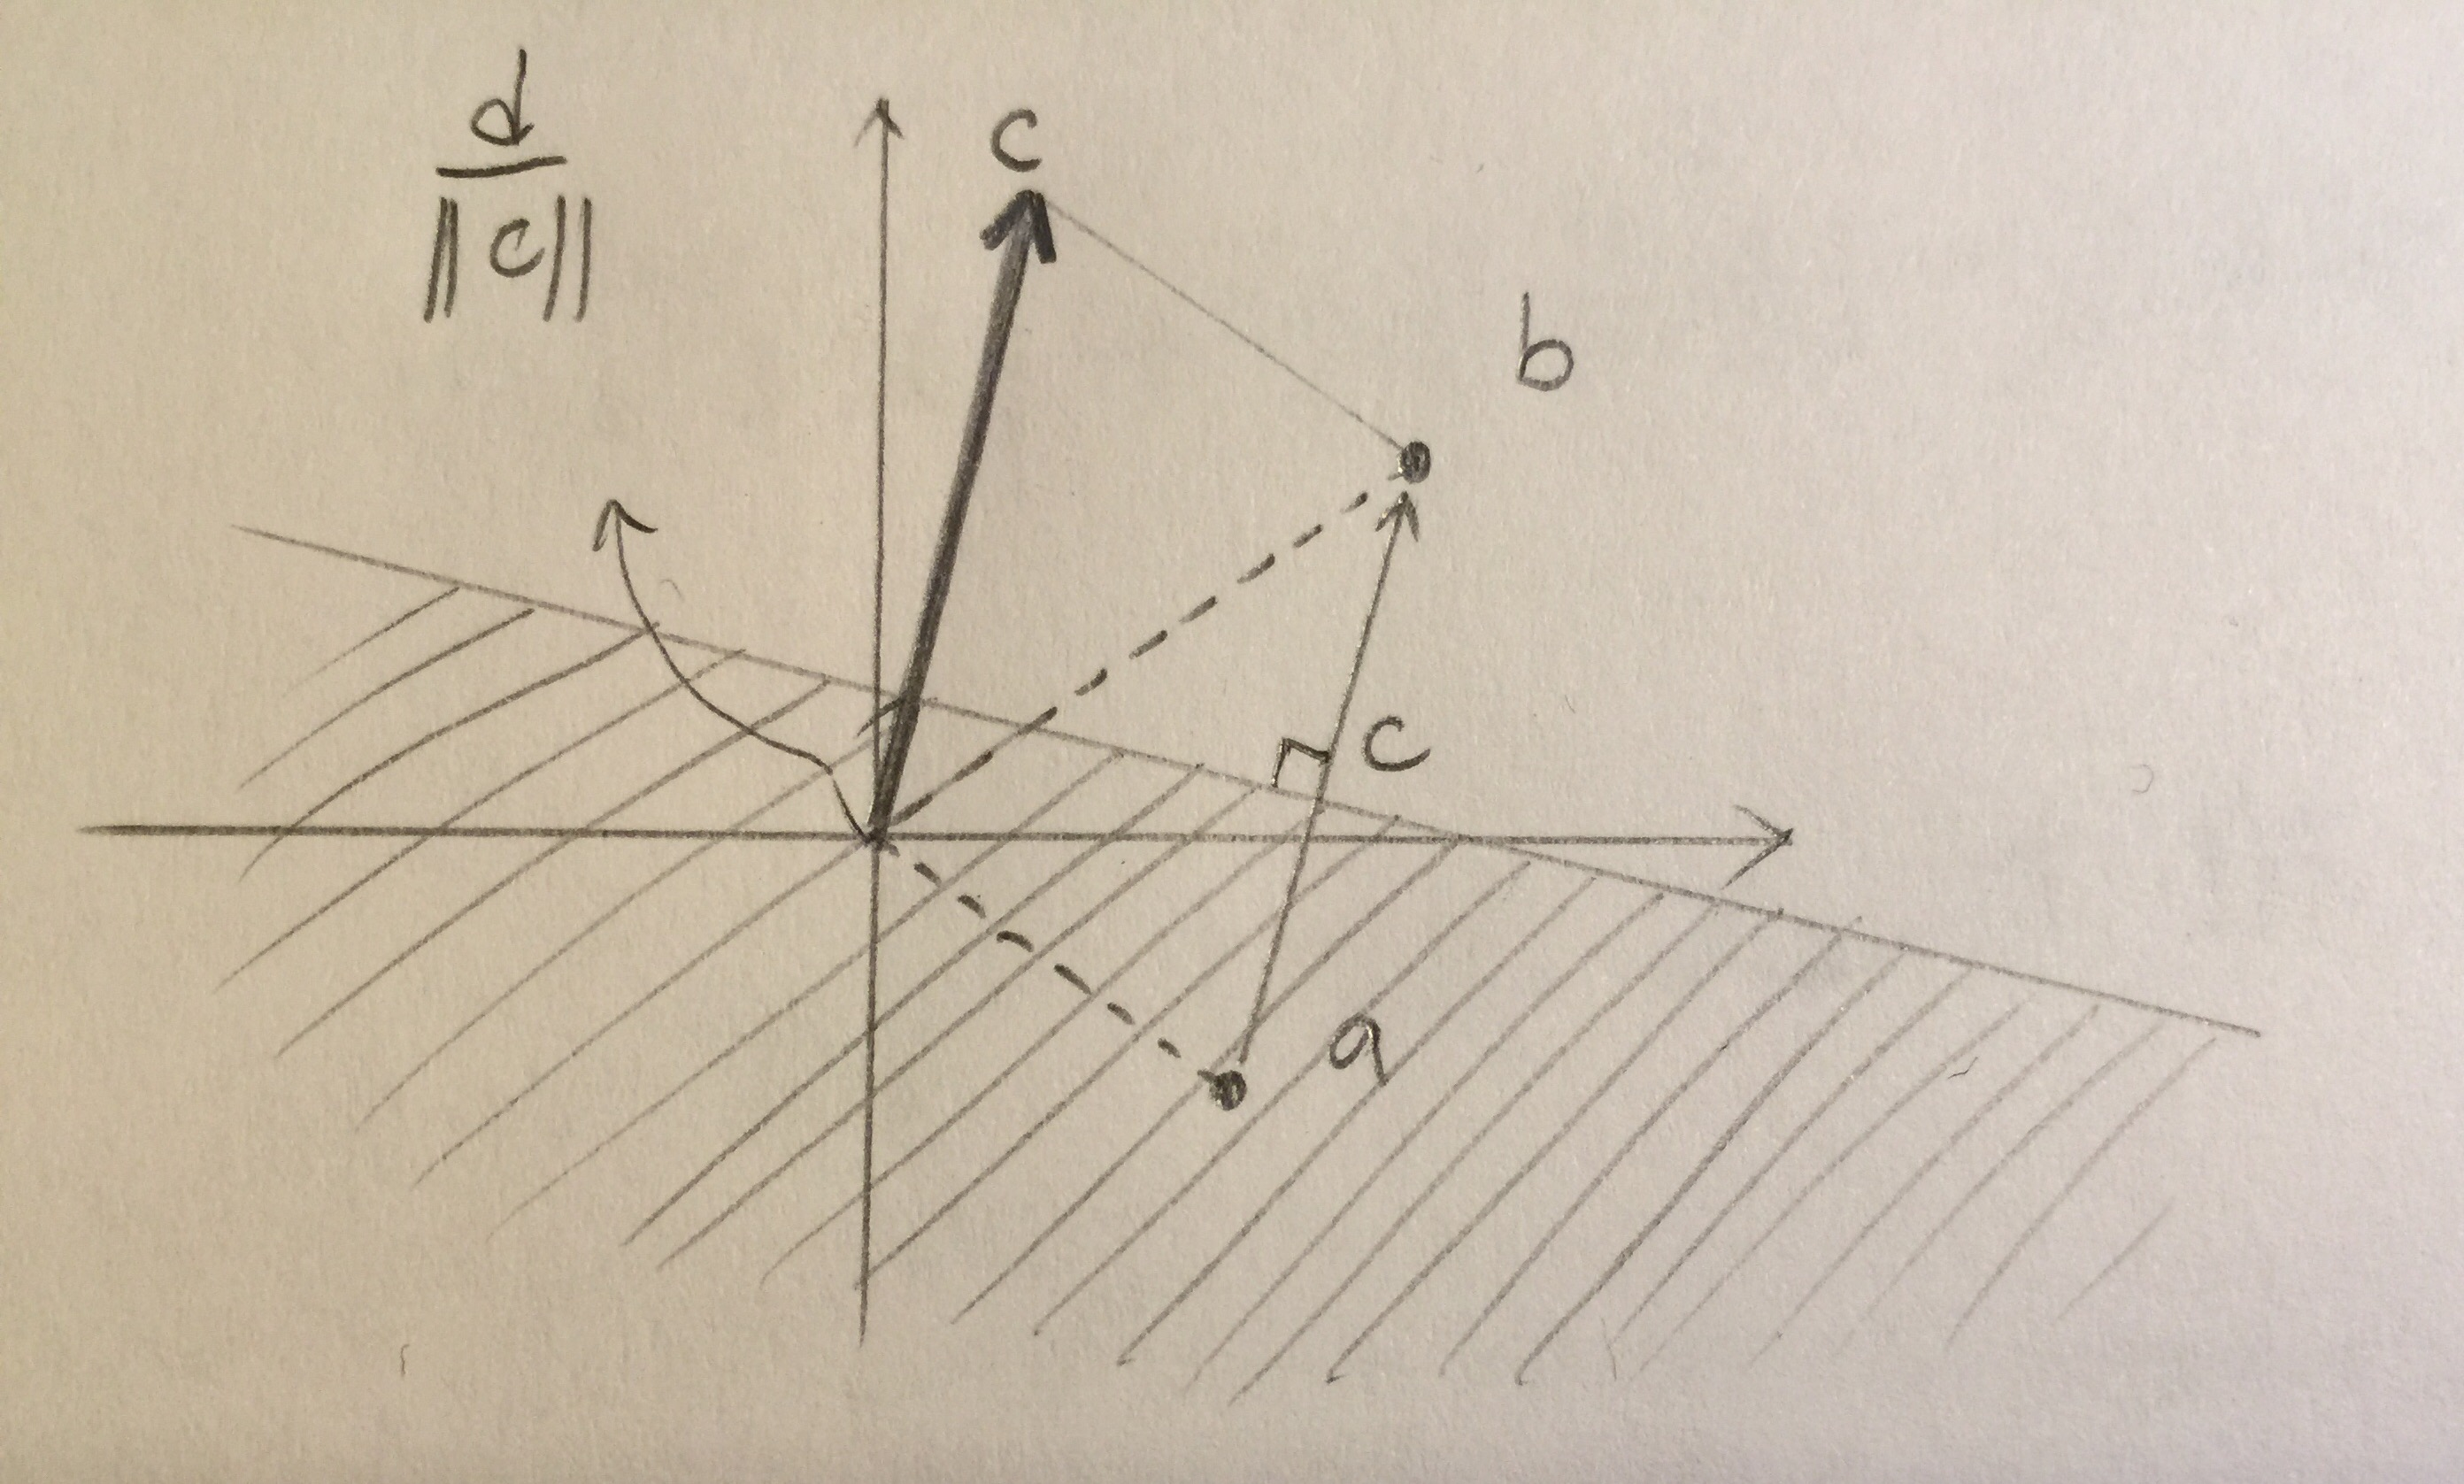
\includegraphics[scale=0.1]{hw1_p1_fig.jpg}
\end{center}



\newpage\subsubsection*{Exercise 2.12 [Boyd \& Vandenberghe, 2004]}
\noindent Which of the following sets are convex? \\
(d) The set of points closer to a given point than a given set, \ie,
$$\{x \mid  \|x-x_0\|_2 \leq \|x-y\|_2 \forall y\in S\}$$
where $S\subseteq \R^n$. \\
\\
{\it Ans:} Observe this set (hereby denoted as $D$) is the intersection of halfspaces (as proved in {\bf 2.7})
$$D = \CAP{y\in S}{} \{x\mid  \|x-x_0\|_2 \leq \|x-y\|_2\}$$
Since intersection of convex sets is also convex, \underline{YES}, the set $D$ is convex. \qed \\
\\
(e) The set of points closer to one set than another, \ie, 
$$\{x \mid  \mbox{dist}(x, S) \leq \mbox{dist}(x, T)\}$$
where $S, T \subseteq \R^n$, and 
$$\mbox{dist}(x, S) = \inf\{\|x-z\|_2 \mid  z\in S\}$$
\\
{\it Ans:} \underline{NO}. Consider counterexample with $S = \{z \mid  \|z\|_2 \geq 2\}$ and $T = \{0\}$; the set described in the problem (hereby denoted as $E$) is the complement set of unit disk
$$E = \{x \mid  \|x\|_2 \geq 1\}$$
This is true since for $x\in\R^n$, $\mbox{dist}(x, \{0\}) = \|x\|_2$ and 
$$\mbox{dist}(x, S) = \casebrak{2-\|x\|_2,\|x\|_2 \leq 2}{0,\|x\|_2 > 2}$$
And certainly the complement set of unit disk is not convex. \qed \\
\\
(f) [HUL93, volume 1, page 93] The set $\{x \mid  x + S_2 \subseteq S_1\}$ where $S_1, S_2 \subseteq \R^n$ with $S_1$ convex. \\
\\
{\it Ans:} \underline{YES}. Take $x_1, x_2 \in F := \{x \mid x + S_2 \subseteq S_1\}$ and arbitrary $y\in S_2$; we have $x_1 + y, x_2 + y \in S_1$ since $x_1, x_2 \in F$. Now for $\theta \in [0, 1]$, since $S_1$ is convex, 
$$\theta(x_1+y) + (1-\theta)(x_2 + y)  = \theta x_1 + (1-\theta)x_2 + y\in S_1$$
Since $y$ was chosen arbitrarily, $\theta x_1 + (1-\theta)x_2 + S_2 \subseteq S_1$; that is, $\theta x_1 + (1-\theta)x_2 \in F$. \qed







\newpage\subsubsection*{Exercise 2.16 [Boyd \& Vandenberghe, 2004]}
\noindent Show that if $S_1$ and $S_2$ are convex sets in \red{$\R^m \x \R^{n}$}\footnote{I believe this was a typo in the textbook.}, then so is their partial sum
$$S = \{(x, y_1+y_2) \mid  x\in \R^m, y_1, y_2 \in \R^n, (x, y_1)\in S_1, (x, y_2)\in S_2\}.$$
\\
{\it Ans:} Take $(x, y_1+y_2), (z, y_3+y_4) \in S$ (where $(x, y_1), (z, y_3) \in S_1, (x, y_2); (z, y_4) \in S_2$) and $\theta \in [0, 1]$; our concern is whether
$$v := \theta (x, y_1+y_2) + (1-\theta)(z, y_3 + y_4) = (\theta x + (1-\theta)z, \theta y_1+(1-\theta)y_3 + \theta y_2 + (1-\theta)y_4)$$
is in $S$. Now that both $S_1$ and $S_2$ are convex, we are safe to claim 
$$\theta (x, y_1) + (1-\theta)(z, y_3) = (\theta x + (1-\theta)z, \theta y_1 + (1-\theta)y_3) \in S_1$$
$$\theta (x, y_2) + (1-\theta)(z, y_4) = (\theta x + (1-\theta)z, \theta y_2 + (1-\theta)y_4) \in S_2$$
Note the vector $v$ is exactly the direct sum of these 2 vectors, henceforth it's in $S$. \qed

\end{document}
